% Options for packages loaded elsewhere
\PassOptionsToPackage{unicode}{hyperref}
\PassOptionsToPackage{hyphens}{url}
\PassOptionsToPackage{dvipsnames,svgnames,x11names}{xcolor}
%
\documentclass[
  11pt,
]{article}
\usepackage{amsmath,amssymb}
\usepackage{iftex}
\ifPDFTeX
  \usepackage[T1]{fontenc}
  \usepackage[utf8]{inputenc}
  \usepackage{textcomp} % provide euro and other symbols
\else % if luatex or xetex
  \usepackage{unicode-math} % this also loads fontspec
  \defaultfontfeatures{Scale=MatchLowercase}
  \defaultfontfeatures[\rmfamily]{Ligatures=TeX,Scale=1}
\fi
\usepackage{lmodern}
\ifPDFTeX\else
  % xetex/luatex font selection
  \setmainfont[]{Latin Modern Roman}
  \setsansfont[]{Latin Modern Sans}
  \setmonofont[]{DejaVu Sans Mono}
\fi
% Use upquote if available, for straight quotes in verbatim environments
\IfFileExists{upquote.sty}{\usepackage{upquote}}{}
\IfFileExists{microtype.sty}{% use microtype if available
  \usepackage[]{microtype}
  \UseMicrotypeSet[protrusion]{basicmath} % disable protrusion for tt fonts
}{}
\makeatletter
\@ifundefined{KOMAClassName}{% if non-KOMA class
  \IfFileExists{parskip.sty}{%
    \usepackage{parskip}
  }{% else
    \setlength{\parindent}{0pt}
    \setlength{\parskip}{6pt plus 2pt minus 1pt}}
}{% if KOMA class
  \KOMAoptions{parskip=half}}
\makeatother
\usepackage{xcolor}
\usepackage[margin=25mm]{geometry}
\usepackage{color}
\usepackage{fancyvrb}
\newcommand{\VerbBar}{|}
\newcommand{\VERB}{\Verb[commandchars=\\\{\}]}
\DefineVerbatimEnvironment{Highlighting}{Verbatim}{commandchars=\\\{\}}
% Add ',fontsize=\small' for more characters per line
\newenvironment{Shaded}{}{}
\newcommand{\AlertTok}[1]{\textcolor[rgb]{1.00,0.00,0.00}{\textbf{#1}}}
\newcommand{\AnnotationTok}[1]{\textcolor[rgb]{0.38,0.63,0.69}{\textbf{\textit{#1}}}}
\newcommand{\AttributeTok}[1]{\textcolor[rgb]{0.49,0.56,0.16}{#1}}
\newcommand{\BaseNTok}[1]{\textcolor[rgb]{0.25,0.63,0.44}{#1}}
\newcommand{\BuiltInTok}[1]{\textcolor[rgb]{0.00,0.50,0.00}{#1}}
\newcommand{\CharTok}[1]{\textcolor[rgb]{0.25,0.44,0.63}{#1}}
\newcommand{\CommentTok}[1]{\textcolor[rgb]{0.38,0.63,0.69}{\textit{#1}}}
\newcommand{\CommentVarTok}[1]{\textcolor[rgb]{0.38,0.63,0.69}{\textbf{\textit{#1}}}}
\newcommand{\ConstantTok}[1]{\textcolor[rgb]{0.53,0.00,0.00}{#1}}
\newcommand{\ControlFlowTok}[1]{\textcolor[rgb]{0.00,0.44,0.13}{\textbf{#1}}}
\newcommand{\DataTypeTok}[1]{\textcolor[rgb]{0.56,0.13,0.00}{#1}}
\newcommand{\DecValTok}[1]{\textcolor[rgb]{0.25,0.63,0.44}{#1}}
\newcommand{\DocumentationTok}[1]{\textcolor[rgb]{0.73,0.13,0.13}{\textit{#1}}}
\newcommand{\ErrorTok}[1]{\textcolor[rgb]{1.00,0.00,0.00}{\textbf{#1}}}
\newcommand{\ExtensionTok}[1]{#1}
\newcommand{\FloatTok}[1]{\textcolor[rgb]{0.25,0.63,0.44}{#1}}
\newcommand{\FunctionTok}[1]{\textcolor[rgb]{0.02,0.16,0.49}{#1}}
\newcommand{\ImportTok}[1]{\textcolor[rgb]{0.00,0.50,0.00}{\textbf{#1}}}
\newcommand{\InformationTok}[1]{\textcolor[rgb]{0.38,0.63,0.69}{\textbf{\textit{#1}}}}
\newcommand{\KeywordTok}[1]{\textcolor[rgb]{0.00,0.44,0.13}{\textbf{#1}}}
\newcommand{\NormalTok}[1]{#1}
\newcommand{\OperatorTok}[1]{\textcolor[rgb]{0.40,0.40,0.40}{#1}}
\newcommand{\OtherTok}[1]{\textcolor[rgb]{0.00,0.44,0.13}{#1}}
\newcommand{\PreprocessorTok}[1]{\textcolor[rgb]{0.74,0.48,0.00}{#1}}
\newcommand{\RegionMarkerTok}[1]{#1}
\newcommand{\SpecialCharTok}[1]{\textcolor[rgb]{0.25,0.44,0.63}{#1}}
\newcommand{\SpecialStringTok}[1]{\textcolor[rgb]{0.73,0.40,0.53}{#1}}
\newcommand{\StringTok}[1]{\textcolor[rgb]{0.25,0.44,0.63}{#1}}
\newcommand{\VariableTok}[1]{\textcolor[rgb]{0.10,0.09,0.49}{#1}}
\newcommand{\VerbatimStringTok}[1]{\textcolor[rgb]{0.25,0.44,0.63}{#1}}
\newcommand{\WarningTok}[1]{\textcolor[rgb]{0.38,0.63,0.69}{\textbf{\textit{#1}}}}
\usepackage{longtable,booktabs,array}
\usepackage{calc} % for calculating minipage widths
% Correct order of tables after \paragraph or \subparagraph
\usepackage{etoolbox}
\makeatletter
\patchcmd\longtable{\par}{\if@noskipsec\mbox{}\fi\par}{}{}
\makeatother
% Allow footnotes in longtable head/foot
\IfFileExists{footnotehyper.sty}{\usepackage{footnotehyper}}{\usepackage{footnote}}
\makesavenoteenv{longtable}
\usepackage{graphicx}
\makeatletter
\def\maxwidth{\ifdim\Gin@nat@width>\linewidth\linewidth\else\Gin@nat@width\fi}
\def\maxheight{\ifdim\Gin@nat@height>\textheight\textheight\else\Gin@nat@height\fi}
\makeatother
% Scale images if necessary, so that they will not overflow the page
% margins by default, and it is still possible to overwrite the defaults
% using explicit options in \includegraphics[width, height, ...]{}
\setkeys{Gin}{width=\maxwidth,height=\maxheight,keepaspectratio}
% Set default figure placement to htbp
\makeatletter
\def\fps@figure{htbp}
\makeatother
\setlength{\emergencystretch}{3em} % prevent overfull lines
\providecommand{\tightlist}{%
  \setlength{\itemsep}{0pt}\setlength{\parskip}{0pt}}
\setcounter{secnumdepth}{5}
% definitions for citeproc citations
\NewDocumentCommand\citeproctext{}{}
\NewDocumentCommand\citeproc{mm}{%
  \begingroup\def\citeproctext{#2}\cite{#1}\endgroup}
\makeatletter
 % allow citations to break across lines
 \let\@cite@ofmt\@firstofone
 % avoid brackets around text for \cite:
 \def\@biblabel#1{}
 \def\@cite#1#2{{#1\if@tempswa , #2\fi}}
\makeatother
\newlength{\cslhangindent}
\setlength{\cslhangindent}{1.5em}
\newlength{\csllabelwidth}
\setlength{\csllabelwidth}{3em}
\newenvironment{CSLReferences}[2] % #1 hanging-indent, #2 entry-spacing
 {\begin{list}{}{%
  \setlength{\itemindent}{0pt}
  \setlength{\leftmargin}{0pt}
  \setlength{\parsep}{0pt}
  % turn on hanging indent if param 1 is 1
  \ifodd #1
   \setlength{\leftmargin}{\cslhangindent}
   \setlength{\itemindent}{-1\cslhangindent}
  \fi
  % set entry spacing
  \setlength{\itemsep}{#2\baselineskip}}}
 {\end{list}}
\usepackage{calc}
\newcommand{\CSLBlock}[1]{\hfill\break\parbox[t]{\linewidth}{\strut\ignorespaces#1\strut}}
\newcommand{\CSLLeftMargin}[1]{\parbox[t]{\csllabelwidth}{\strut#1\strut}}
\newcommand{\CSLRightInline}[1]{\parbox[t]{\linewidth - \csllabelwidth}{\strut#1\strut}}
\newcommand{\CSLIndent}[1]{\hspace{\cslhangindent}#1}
\usepackage{fancyhdr}
\usepackage{microtype}
\usepackage{needspace}
\usepackage{float}
\usepackage{caption}
\usepackage{seqsplit}
\captionsetup{font=small,labelfont=bf}
\floatplacement{figure}{H}
\pagestyle{fancy}
\fancyhf{}
\fancyhead[L]{\footnotesize\textsc{TACITUS · Context capsules}}
\fancyhead[R]{\footnotesize Research proposal TAC-2026-01 · v1.0}
\fancyfoot[C]{\small\thepage}
\setlength{\headheight}{14pt}
\setlength{\emergencystretch}{3em}
\setlength{\parskip}{5pt}
\setlength{\parindent}{0pt}
\AtBeginEnvironment{CSLReferences}{\interlinepenalty=10000}
\renewcommand{\headrulewidth}{0.3pt}
\AtBeginDocument{\hypersetup{pdftitle={TACITUS: Context Capsules, Artefacts, and Small Knowledge Graphs for AI Generation},pdfauthor={TACITUS},pdfsubject={Research proposal TAC-2026-01, version 1.0; not independently peer-reviewed},pdfkeywords={context capsules, artefacts, knowledge graphs, provenance, generation, evaluation}}}
\let\originalsection\section
\renewcommand{\section}{\Needspace{5\baselineskip}\originalsection}
\ifLuaTeX
  \usepackage{selnolig}  % disable illegal ligatures
\fi
\usepackage{bookmark}
\IfFileExists{xurl.sty}{\usepackage{xurl}}{} % add URL line breaks if available
\urlstyle{same}
\hypersetup{
  pdftitle={TACITUS: Context Capsules, Artefacts, and Small Knowledge Graphs for AI Generation},
  pdfauthor={TACITUS},
  colorlinks=true,
  linkcolor={teal},
  filecolor={Maroon},
  citecolor={Blue},
  urlcolor={teal},
  pdfcreator={LaTeX via pandoc}}

\title{TACITUS: Context Capsules, Artefacts, and Small Knowledge Graphs
for AI Generation}
\author{TACITUS}
\date{23 November 2026}

\begin{document}
\maketitle
\begin{abstract}
Knowledge work depends on more than retrieving a relevant document. A
useful answer may also require the conditions attached to a claim, the
reason a team chose particular language, an unresolved objection, and an
earlier decision about the intended audience. This paper proposes an
architecture and evaluation program for TACITUS App, a conversation and
writing workspace in which teams attach reusable context capsules and
artefacts. A capsule packages selected, versioned sources, working
instructions, qualifications, and inspectable interpretations. A small
knowledge graph records typed relationships among these materials; a
bounded projection, rather than the entire graph, enters generation.
Artefacts provide reusable formats and examples and retain links to the
context of their production. We describe evidence anchoring, semantic
layers, human review, context compilation, and transfer between people
and agents, distinguishing implemented reference contracts from proposed
capabilities. Six previously recorded provider probes illustrate both
preserved conditions and a graph-associated status error; they do not
establish an improvement in generation quality. We specify a controlled
comparison against passage retrieval, a representation ablation, and a
team-handover study, with claim support, critical qualifications,
abstention, review effort, and total cost as outcomes. The central
hypothesis is that explicit, reviewable context can improve useful
generation and continuity. Its benefit, optimal graph size, and economic
value remain empirical questions.
\end{abstract}

\textbf{Research proposal TAC-2026-01 · Version 1.0.} Published by
TACITUS. This proposal has not undergone independent peer review. The
confirmatory experiments described here have not been run or
preregistered.

\textbf{Keywords:} retrieval-augmented generation; context engineering;
knowledge graphs; provenance; collaborative writing; organizational
memory; human--AI interaction.

\section{Introduction}\label{introduction}

A colleague preparing a policy analysis often needs to know why an
earlier draft used ``may'' rather than ``will,'' which source edition
supports the distinction, who objected to an interpretation, and what
remains unresolved. A new conversation with an AI assistant usually
begins with a question and a subset of documents. Relevant working
context can remain in another conversation, a meeting note, an annotated
draft, or a teammate's memory. The resulting answer may be fluent and
correctly cite a passage while omitting the condition that makes its
recommendation defensible.

TACITUS App is organized around a simple interaction: start a
conversation or draft, attach context capsules and artefacts, inspect
what will be supplied, and reuse that context in later work. The company
website presents the technology; the authenticated application is the
workspace. A capsule is a reusable package of working context. An
artefact is an input or output work product, such as a template,
example, analytical note, or saved answer. A small graph connects their
selected sources, interpretations, qualifications, and discussion
records. These relationships are intended to make context easier to
carry, inspect, and revise.

The research question is whether this organization improves generation
relative to a strong model with ordinary document retrieval, after
accounting for the work required to construct and maintain it. The
proposed mechanism has three parts. First, explicit dependencies can
keep a claim with its conditions and counterevidence. Second, versioned
context can preserve team decisions across conversations and handovers.
Third, task-bounded selection can give a model relevant material without
indiscriminately adding the whole organizational archive. Each mechanism
can fail: an annotation can be wrong, a graph can omit dissent, and
selection can discard essential evidence.

The contribution is an inspectable system design and a falsifiable
evaluation proposal, supported by an existing open reference
implementation and limited recorded provider observations. It is not a
new foundation model, a claim to have invented graph retrieval, or an
empirical demonstration of superior accuracy. The principal question
concerns useful work: whether an analyst reaches a supported,
appropriately qualified output with less total effort, and whether
another person or agent can continue it without reconstructing the
context.

\section{Related work and research
position}\label{related-work-and-research-position}

\subsection{Retrieval, graphs, and context
selection}\label{retrieval-graphs-and-context-selection}

Retrieval-augmented generation combines a generator with external
retrievable information (\citeproc{ref-lewis2020}{Lewis et al. 2020}).
This motivates keeping evidence outside model parameters, but attaching
documents alone does not specify how a team's decisions and
qualifications should travel with an answer. BM25 provides a strong,
reproducible lexical retrieval baseline
(\citeproc{ref-robertson2009}{Robertson and Zaragoza 2009}). It should
be included in evaluation rather than assuming that a graph necessarily
adds value.

Long-context experiments show that the position of relevant material can
affect a model's ability to use it (\citeproc{ref-liu2024}{Liu et al.
2024}). These findings motivate positional and budget stress tests. They
do not prove that every shorter prompt performs better, or that the same
effect size applies to a later model. TACITUS treats salience as
task-specific retention and use of consequential information, rather
than an intrinsic property of a visually prominent node.

GraphRAG constructs an entity graph and community summaries for
corpus-level, query-focused summarization (\citeproc{ref-edge2024}{Edge
et al. 2024}). HippoRAG combines knowledge graphs and Personalized
PageRank for knowledge integration and multi-hop retrieval
(\citeproc{ref-gutierrez2024}{Jiménez Gutiérrez et al. 2024}). LightRAG
uses graph and vector representations with retrieval at different levels
and incremental updates (\citeproc{ref-guo2025}{Guo et al. 2025}). These
are related approaches with different algorithms and evaluation
settings. TACITUS's reviewed reference uses explicit authored mappings
and bounded selection; it does not reproduce those systems' algorithms
or inherit their results. Its proposed unit is a portable context
package for a task and a team, which can be used with lexical, vector,
or graph-based retrieval.

Self-RAG demonstrates a learned approach to conditional retrieval and
reflection (\citeproc{ref-asai2024}{Asai et al. 2024}). ReAct studies
interleaving model reasoning and task actions
(\citeproc{ref-yao2023}{Yao et al. 2023}). They motivate investigating
when evidence access or another check is useful. A fixed verification
stage in TACITUS is not a trained reflection policy, and multiple model
stages do not supply independent corroboration.

\subsection{Attribution, memory, and
review}\label{attribution-memory-and-review}

ALCE evaluates generation along distinct dimensions including
correctness and citation quality (\citeproc{ref-gao2023}{Gao et al.
2023}). Attributable to Identified Sources separates a statement's
interpretation from whether supplied evidence supports it
(\citeproc{ref-rashkin2023}{Rashkin et al. 2023}). FActScore shows the
importance of evaluating individual factual claims within a longer
answer (\citeproc{ref-min2023}{Min et al. 2023}). Accordingly, this
proposal distinguishes a resolving citation identifier, a faithful
quotation, and a supported generated claim. Passing the first two checks
does not establish the third.

LongMemEval evaluates information extraction, reasoning across sessions,
temporal reasoning, knowledge updates, and abstention
(\citeproc{ref-wu2025}{Wu et al. 2025}). These abilities are relevant to
context handover. A bounded, explicitly attached capsule differs from an
assistant automatically remembering its entire interaction history. The
evaluation must test both continuity and whether obsolete or
unauthorized context is excluded.

PROV-O provides a vocabulary for provenance, and SHACL specifies
validation of RDF graphs against declared constraints
(\citeproc{ref-prov2013}{Lebo, Sahoo, and McGuinness 2013};
\citeproc{ref-shacl2017}{Knublauch and Kontokostas 2017}). They inform
the separation of records, transformations, and responsibilities. The
present JSON and JSON-LD reference contracts do not establish full
PROV-O conformance or implement a general SHACL reasoner. Application
validation checks declared structural conditions; it does not prove the
truth of an interpretation.

Human--AI interaction guidelines motivate understandable system
behavior, correction, and control over adaptation
(\citeproc{ref-amershi2019}{Amershi et al. 2019}). Model cards motivate
explicit reporting of intended use, evaluation, and limitations
(\citeproc{ref-mitchell2019}{Mitchell et al. 2019}). Finally, plausible
model explanations can be unfaithful to the process that produced a
prediction (\citeproc{ref-turpin2023}{Turpin et al. 2023}). The
``reasoning'' preserved by TACITUS therefore means shareable human
discussion, explicit analytical warrants, objections, and attributed
model summaries. It is not a claim to reveal or authenticate a model's
hidden chain of thought.

\section{System model}\label{system-model}

\subsection{Context capsules and
artefacts}\label{context-capsules-and-artefacts}

A capsule binds a purpose and scope to selected context. Its proposed
general contract includes the task audience, working instructions, exact
source editions, interpretations and their review records, mandatory
conditions, unresolved questions, and expiry or refresh rules. Reuse
should preserve the identities and versions of these components. A
capsule is not automatically a verified statement about the world:
different fields can contain evidence, instructions, or a team's
provisional position.

An artefact can be attached as an example or format to follow. It can
also be the result of generation or human writing. The two roles require
different treatment. An example can guide structure without establishing
that its factual content applies to the new task. A newly generated
artefact should retain the selected context receipt, model and execution
settings, output version, and subsequent human edits. Applying a
suggested revision should remain an explicit writing operation.

\begin{longtable}[]{@{}
  >{\raggedright\arraybackslash}p{(\columnwidth - 4\tabcolsep) * \real{0.3333}}
  >{\raggedright\arraybackslash}p{(\columnwidth - 4\tabcolsep) * \real{0.3333}}
  >{\raggedright\arraybackslash}p{(\columnwidth - 4\tabcolsep) * \real{0.3333}}@{}}
\caption{Record types have different evidentiary roles. A discussion is
evidence that a contribution was recorded, not proof of its substantive
claim. A human review records a judgment within a scope, not universal
certification.}\tabularnewline
\toprule\noalign{}
\begin{minipage}[b]{\linewidth}\raggedright
Record
\end{minipage} & \begin{minipage}[b]{\linewidth}\raggedright
Necessary distinction
\end{minipage} & \begin{minipage}[b]{\linewidth}\raggedright
Example in analytical work
\end{minipage} \\
\midrule\noalign{}
\endfirsthead
\toprule\noalign{}
\begin{minipage}[b]{\linewidth}\raggedright
Record
\end{minipage} & \begin{minipage}[b]{\linewidth}\raggedright
Necessary distinction
\end{minipage} & \begin{minipage}[b]{\linewidth}\raggedright
Example in analytical work
\end{minipage} \\
\midrule\noalign{}
\endhead
\bottomrule\noalign{}
\endlastfoot
Source and passage & Exact edition and quotation, separate from
interpretation & The adopted wording of a conditional permission \\
Claim or interpretation & Attributed proposition with scope and review
state & An analyst's reading of the permission \\
Qualification & Condition, exception, modality, time, or jurisdiction &
Renewal requires an independent review \\
Discussion or warrant & A recorded contribution and its stated role &
Why the team retained conditional language \\
Capsule & Reusable selection and working guidance & How this team
prepares a decision note \\
Artefact & Versioned example, format, draft, or result & A template or a
source-linked analytical paragraph \\
Execution receipt & Actual selected inputs and observed execution & What
a particular generation request received \\
\end{longtable}

\subsection{A bounded, layered graph}\label{a-bounded-layered-graph}

Let a case graph be \(G=(V,E)\) with typed nodes and edges. ``Small
graph'' or ``micrograph'' denotes a task-scoped projection with explicit
bounds, not a universal node-count threshold or a distinct mathematical
graph class. The complete case graph can be larger than the material
sent to a model. A display containing hundreds of points is not, by
itself, a richer evidentiary structure.

Six layers are useful. The \textbf{source layer} identifies documents,
editions, passages, and their lineage. The \textbf{ontology layer}
declares entity types and permitted relationships, such as an
institution issuing a statement or a qualification limiting a claim. The
\textbf{assertion layer} represents attributed interpretations,
modality, conditions, time, and disagreement. The \textbf{deliberation
layer} records working decisions, objections, and stated warrants. The
\textbf{task layer} selects the current question, audience, capsule, and
artefact requirements. The \textbf{execution layer} records the context
actually dispatched and the resulting work product. The layers
distinguish purposes; they need not require separate databases.

An ontology supplies a vocabulary and constraints. A semantic layer
applies that vocabulary to a particular analytical task, selecting
relevant assertions and review checks. Neither adds missing evidence.
Entity resolution should retain distinct identities when names coincide;
a quoted position of an organization should not become a user's personal
belief. An authored ``supports'' edge is an interpretation that can be
challenged. It is not an independent observation or a probability of
truth.

\begin{figure}
\centering
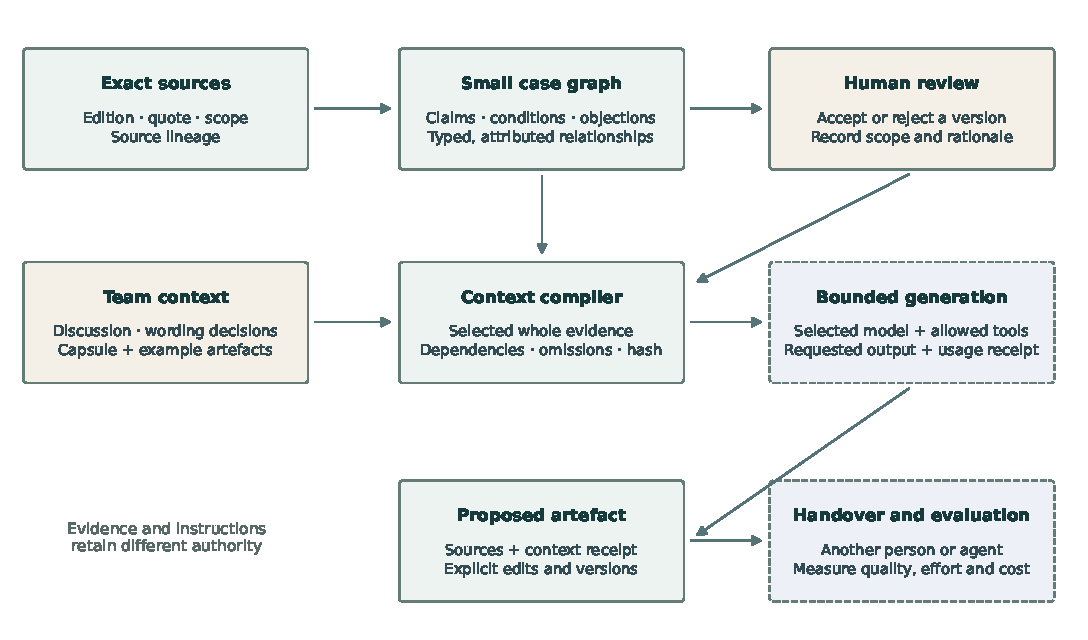
\includegraphics{figures/context-flow.pdf}
\caption{Proposed information flow. Source material and team decisions
retain separate roles. The context compiler selects a bounded package;
generation produces a proposed artefact, and human revision creates
another version. Solid boxes indicate record and compilation contracts;
dashed boxes indicate capabilities or integrations that require further
evaluation.}
\end{figure}

\subsection{Review and changes over
time}\label{review-and-changes-over-time}

The proposed lifecycle distinguishes a captured source, an authored or
model-proposed interpretation, a scoped human acceptance, and later
rejection, revocation, or supersession. The public reference
intentionally emits interpretations as proposed; it cannot grant human
approval. The App has separate interpretation-review and
graph-activation contracts. Accepting an interpretation should not
silently activate an entire graph, and an automated critic should not
impersonate human review.

Review must bind to exact content and dependencies. A reviewer should
see the relevant passage, interpretation, qualifications, and intended
use before accepting a version. A new source edition can invalidate a
dependency without erasing the historical record. Existing frozen
receipts should remain identifiable, while new dispatch checks current
access, active versions, and review state. A shared historical packet
cannot be made confidential again merely by revoking later access;
retention, export, and deletion need explicit operational policies.

\section{Context compilation and
generation}\label{context-compilation-and-generation}

\subsection{Selection with required
dependencies}\label{selection-with-required-dependencies}

For a task \(q\), let \(S\) be candidate selected records, \(R_q\) the
mandatory task records, and \(\operatorname{cl}_G(S)\) their declared
dependency closure. Closure includes the exact support spans, necessary
conditions, and known linked objections required to interpret the
selected claims. Let \(b(\cdot)\) measure the serialized input size. A
design objective is

\[
S_q^* = \arg\max_S U(q,S),\qquad
R_q\subseteq S,\quad b(\operatorname{cl}_G(S))\leq B.
\]

Here \(U\) is a proposed task-utility objective, not an implemented
learned score or proven optimum. The current reference uses
deterministic selection and whole-statement packing; the App includes
lexical matching, selected graph anchors, and adjacent-qualification
handling. These are engineering heuristics. They can preserve declared
dependencies but cannot discover every relevant exception in an unseen
corpus. Known critical information should be explicit in the contract,
and missing information should remain visible.

The compiler should validate access and version pins, retrieve eligible
material, expand only within declared bounds, retain required
dependencies, and serialize the selected context with an omission
report. If mandatory evidence does not fit, the request should fail or
ask for a narrower scope rather than silently truncating the condition.
Optional material can be omitted with an explanation. The full graph and
the generation packet are distinct outputs.

Bounds are implementation controls, not scientific findings. In the
reviewed App graph-context contract, selections are limited to four
graphs, 128 nodes, 256 edges, 24 KiB of graph context, and 65,536 bytes
for the complete packet. The reference pipeline has its own byte budgets
and selection options, including graph expansion limited to two hops.
These values do not imply an optimal context size. Bytes, model tokens,
graph records, and billed tokens are different quantities and must be
measured separately.

\subsection{Generation and source
checking}\label{generation-and-source-checking}

The same frozen packet should be usable in Conversation and Writing. A
dispatch receipt should identify source and object versions, selected
graph records, the packet checksum, requested and reported model
identity, settings, and observed usage. Switching a model should not
change which source version a previous request used. Hosted and local
models require the same evidence and output contracts, while their
inference, retention, resource, and failure characteristics differ.

A useful checking sequence separates four questions: does the quotation
match the pinned source; does the citation identifier resolve; does the
claim preserve the source's scope and modality; and is the final
analysis adequate for its purpose? Exact-span and schema checks can be
deterministic. Entailment, applicability, and substantive judgment
require evaluated methods and human assessment. A source check should
therefore report the operation performed and its limits, rather than
displaying a general trust score.

In the writing interface, a reader should be able to select a supported
phrase and inspect its source span, interpretation, objections, and
revision history. Operations such as checking a paragraph, challenging a
conclusion, applying a changed source edition, or requesting a
teammate's criticism can share this record model. They should create
attributed proposals rather than silently alter a saved document. These
interface and workflow extensions are design proposals where not already
covered by the reviewed source contracts.

\subsection{Bounded agents and human
handover}\label{bounded-agents-and-human-handover}

An agent can receive the same packet as a colleague, together with a
finite task and allowed tools. The public reference includes a bounded
evidence-inspection and drafting loop. A production extension should
identify each tool input, result, dependency, and uncertain completion
state. A second model report is another generated interpretation of the
evidence, not a new source. A retry after an uncertain provider outcome
must not silently create a duplicate paid execution.

The handover packet should answer what is being attempted, what material
supports it, why particular wording was chosen, which alternatives were
considered, what remains disputed, and what the next actor may do. A
persona is a declared analytical lens or authorized writing instruction.
It should not claim that a named person or organization endorsed a
generated judgment. The intended contribution is continuity of explicit
work context, not imitation of an individual's private beliefs.

\section{Inspectable example and current
implementation}\label{inspectable-example-and-current-implementation}

\subsection{A conditional permission and a recorded
objection}\label{a-conditional-permission-and-a-recorded-objection}

Consider two synthetic source records from the existing provider probe.
One states: ``The board may renew the licence for six months only if the
independent reviewer accepts the risk note.'' The other records an
objection that the risk note is incomplete and no final renewal
approval. A generated statement that renewal was approved would be
unsupported. A statement that renewal was ``only proposed'' also
introduces a procedural status not established by the conditional
permission alone.

The accompanying executable demonstration adds a clearly labelled
authored discussion about keeping the condition and objection with the
recommendation. It creates proposed, qualified mappings using the public
reference tool. Figure 2 shows the conceptual relationships. The
compiler retains source identity, quotation, condition, and the
discussion's role. The demonstration is an original synthetic fixture,
not a real organization, legal opinion, human-approved capsule, or
generated customer deliverable.

\begin{figure}
\centering
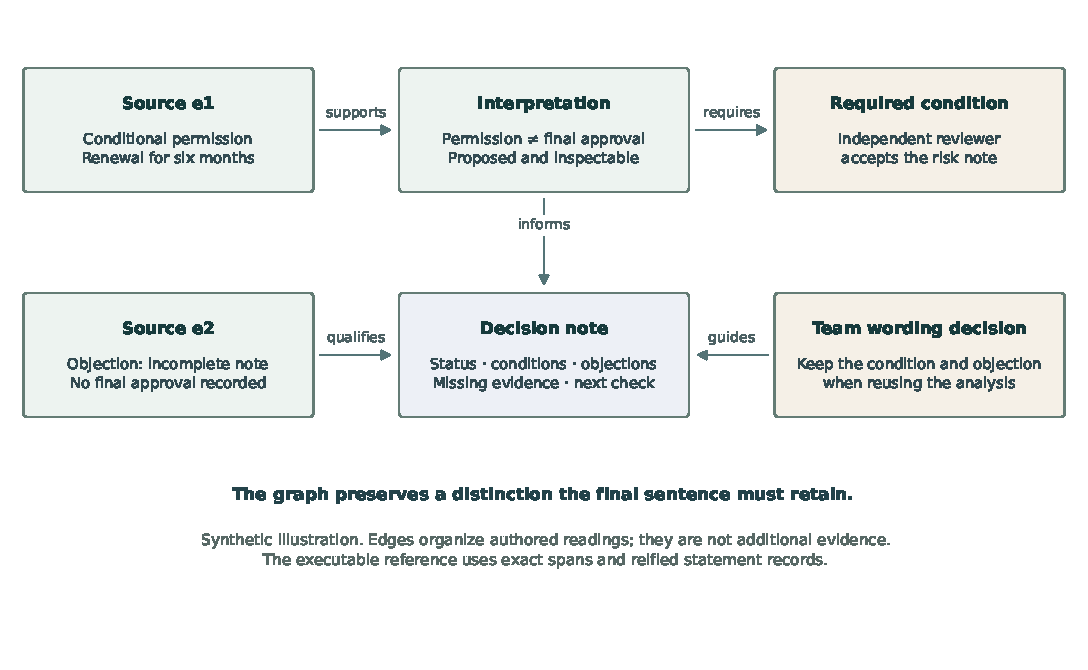
\includegraphics{figures/qualified-context.pdf}
\caption{A conceptual small graph for the synthetic renewal example. A
permission, condition, recorded objection, team wording decision, and
output format retain different types. The dotted team-guidance
relationship does not establish a source fact. The executable graph uses
the reference format's reified statements and exact spans; the diagram
simplifies that representation.}
\end{figure}

An appropriate source-limited analytical sentence would preserve the
conditional permission, the six-month duration, the objection, and the
absence of recorded final approval. This sentence is an authored target
illustration, not a newly measured model result. A handover should also
preserve the team's stated reason for cautious wording, so another
writer can adapt the text without losing that distinction.

\subsection{Implemented contracts and operational
boundary}\label{implemented-contracts-and-operational-boundary}

The inspected open pipeline validates exact UTF-8 source editions,
Unicode code-point quotation spans, declared qualifier literals, and
ontology domain/range. It emits graph JSON, JSON-LD, bounded capsules,
an evidence worksheet, and checksum receipts. The App import adapter
validates its package and converts source offsets to the App's UTF-16
convention. Graph and capsule records remain separately versioned.

The reviewed App source contains attachment previews and receipts, saved
capsules and artefacts, graph selection, interpretation review, private
team adaptation, model selection, and local-companion contracts. An
authored catalogue method graph represents the requirements of a method;
its input slots are not completed source evidence. This paper does not
treat catalogue size, graph density, screenshots, or automated tests as
evidence that customers obtain better analyses.

The documented hosted release keeps generation paused. In particular, a
configured provider or billing guard is not an accepted end-to-end
inference route. This proposal does not activate generation, reroute
billing, execute paid model calls, or claim new production acceptance.
Implementation descriptions refer to the pinned source review in
Appendix A; they are not a fresh independent audit of every deployed
feature.

\begin{longtable}[]{@{}
  >{\raggedright\arraybackslash}p{(\columnwidth - 4\tabcolsep) * \real{0.3333}}
  >{\raggedright\arraybackslash}p{(\columnwidth - 4\tabcolsep) * \real{0.3333}}
  >{\raggedright\arraybackslash}p{(\columnwidth - 4\tabcolsep) * \real{0.3333}}@{}}
\caption{Implementation, compatibility, and efficacy are different
levels of evidence. The publication builder replays the synthetic
demonstration and verifies existing record hashes without
inference.}\tabularnewline
\toprule\noalign{}
\begin{minipage}[b]{\linewidth}\raggedright
Component
\end{minipage} & \begin{minipage}[b]{\linewidth}\raggedright
Evidence available for this proposal
\end{minipage} & \begin{minipage}[b]{\linewidth}\raggedright
Boundary
\end{minipage} \\
\midrule\noalign{}
\endfirsthead
\toprule\noalign{}
\begin{minipage}[b]{\linewidth}\raggedright
Component
\end{minipage} & \begin{minipage}[b]{\linewidth}\raggedright
Evidence available for this proposal
\end{minipage} & \begin{minipage}[b]{\linewidth}\raggedright
Boundary
\end{minipage} \\
\midrule\noalign{}
\endhead
\bottomrule\noalign{}
\endlastfoot
Source validation and bounded assembly & Executable public Python
reference and tests & Authored mappings; no automatic semantic truth \\
Capsule and graph interchange & Public format and private App adapter
source & Import validation is distinct from human acceptance \\
Conversation and Writing context & Reviewed App contracts and
documentation & Production generation remains gated in the documented
release \\
Model compatibility & Six recorded direct provider responses & One
synthetic task; no App dispatch acceptance \\
General generation-quality improvement & Evaluation protocol proposed
below & No confirmatory result is available \\
Team productivity and paid value & Handover and cost study proposed
below & No observed customer-time or revenue effect \\
\end{longtable}

\subsection{Limited provider
observations}\label{limited-provider-observations}

On 23 November 2026 UTC, an earlier compatibility exercise made six
direct Cloudflare Workers AI REST requests: flat and graph-annotated
context for three reported model families. All six returned schema-valid
final answers with resolving citation identifiers. The paired arms used
the same two source records, question, and output cap, but the graph arm
added annotations. These are not information-equivalent or token-matched
comparisons.

\begin{longtable}[]{@{}
  >{\raggedright\arraybackslash}p{(\columnwidth - 4\tabcolsep) * \real{0.3333}}
  >{\raggedright\arraybackslash}p{(\columnwidth - 4\tabcolsep) * \real{0.3333}}
  >{\raggedright\arraybackslash}p{(\columnwidth - 4\tabcolsep) * \real{0.3333}}@{}}
\caption{Qualitative observations from the existing six-response record.
Review was post-hoc, unblinded, and performed with AI assistance; it was
not independent domain review. Exact provider identifiers and final
answers remain in the public receipts.}\tabularnewline
\toprule\noalign{}
\begin{minipage}[b]{\linewidth}\raggedright
Recorded model family
\end{minipage} & \begin{minipage}[b]{\linewidth}\raggedright
Flat context
\end{minipage} & \begin{minipage}[b]{\linewidth}\raggedright
Graph-annotated context
\end{minipage} \\
\midrule\noalign{}
\endfirsthead
\toprule\noalign{}
\begin{minipage}[b]{\linewidth}\raggedright
Recorded model family
\end{minipage} & \begin{minipage}[b]{\linewidth}\raggedright
Flat context
\end{minipage} & \begin{minipage}[b]{\linewidth}\raggedright
Graph-annotated context
\end{minipage} \\
\midrule\noalign{}
\endhead
\bottomrule\noalign{}
\endlastfoot
Gemma 4 & Omitted the requested reviewer condition & Preserved
condition, duration, objection, and absence of approval \\
GPT-OSS 120B & Preserved the material qualifications & Preserved the
material qualifications \\
GLM 5.3 & Preserved the material qualifications & Added ``only
proposed'' and omitted the duration \\
\end{longtable}

The structured annotation labelled the renewal a proposed action. Its
possible influence on the stronger status wording is a useful failure
hypothesis, not an identified causal effect. Schema validity and
resolving citations did not prevent a substantive omission or status
error. One task and one response per arm cannot estimate average
benefit, statistical uncertainty, or behavior on later model releases.
The publication makes no quality leaderboard from these observations.

\section{Proposed evaluation}\label{proposed-evaluation}

\subsection{Questions, tasks, and
controls}\label{questions-tasks-and-controls}

The primary hypothesis is that the complete reviewed-context pipeline
improves \textbf{clean task completion} over passage retrieval for tasks
requiring qualifications or continuity. A second hypothesis concerns
whether graph organization adds value beyond the same reviewed
information rendered as a flat packet. A third asks whether saved
context reduces handover effort without increasing consequential error.
Each can be rejected independently.

An initial feasibility study should use at least 24 tasks across
disjoint source collections. A provisional confirmatory design is 120
tasks from 30 collections, with the final sample size set through
clustered power analysis using feasibility data before the test set is
unlocked. The numbers are proposed planning quantities, not an adequacy
claim or a completed study. A protocol, stopping rule, primary
comparison, and exclusions must be registered before confirmatory
execution.

Tasks should cover analytical writing, source comparison, conditional
rules, conflicting accounts, edition changes, multilingual wording,
prior team discussion, and insufficient evidence. Include policy and
political work, but also other knowledge tasks to test the generic
workspace design. An independent panel should create held-out questions,
critical points, and reference judgments. Graph builders should not see
the held-out answers or tune annotations to failed test outputs. Freeze
case-level annotations and capsule definitions before question
disclosure; record any task-time selection as part of the evaluated
pipeline.

The same model snapshot, source pool, question, system instructions,
answer format, decoding settings, and output cap should be held fixed
within each paired comparison. Model choice is a blocked factor. A
hosted model and a runnable local model can test portability after their
actual routes and resource settings are recorded. A model change
requires another block, not an unreported substitution. Separate tasks
that fit a full-document baseline from tasks whose corpus exceeds the
model's context limit, using a rule fixed before outcomes are observed.

\begin{longtable}[]{@{}
  >{\raggedright\arraybackslash}p{(\columnwidth - 4\tabcolsep) * \real{0.3333}}
  >{\raggedright\arraybackslash}p{(\columnwidth - 4\tabcolsep) * \real{0.3333}}
  >{\raggedright\arraybackslash}p{(\columnwidth - 4\tabcolsep) * \real{0.3333}}@{}}
\caption{Proposed experimental arms. C and D must retain equivalent
stated information; the flat rendering must not discard a relation's
meaning merely to create a weak comparator. Prompt lengths may differ
and must be reported. The D--B contrast measures the complete pipeline,
including annotation work, rather than a graph-only causal
effect.}\tabularnewline
\toprule\noalign{}
\begin{minipage}[b]{\linewidth}\raggedright
Arm
\end{minipage} & \begin{minipage}[b]{\linewidth}\raggedright
Input construction
\end{minipage} & \begin{minipage}[b]{\linewidth}\raggedright
Comparison supported
\end{minipage} \\
\midrule\noalign{}
\endfirsthead
\toprule\noalign{}
\begin{minipage}[b]{\linewidth}\raggedright
Arm
\end{minipage} & \begin{minipage}[b]{\linewidth}\raggedright
Input construction
\end{minipage} & \begin{minipage}[b]{\linewidth}\raggedright
Comparison supported
\end{minipage} \\
\midrule\noalign{}
\endhead
\bottomrule\noalign{}
\endlastfoot
A: full documents & Pinned source text, within a declared eligible limit
& Whether selective context helps on the common eligible subset \\
B: passage retrieval & Frozen lexical retrieval and ordinary source
metadata & Primary practical baseline \\
C: reviewed flat context & The same selected evidence, instructions, and
reviewed propositions as D, expressed linearly & Whether reviewed
content helps without graph serialization \\
D: capsule and micrograph & The reviewed packet with explicit typed
relationships and dependencies & Complete pipeline versus B;
representation diagnostic versus C \\
\end{longtable}

\subsection{Outcomes and analysis}\label{outcomes-and-analysis}

Before generation, reviewers should list the task's critical facts,
required qualifications, expected treatment of uncertainty, and
acceptable abstentions. For task \(i\) and arm \(a\), define

\[
\mathrm{Clean}_{ia} = \mathbf{1}\{\text{valid completion, all critical points handled, no consequential unsupported claim}\}.
\]

An invalid, refused, missing, or timed-out output does not pass
assigned-task completion. A justified abstention can pass when the
reference rubric requires it. This prevents a method from improving its
apparent precision by silently dropping difficult tasks. The primary
paired effect is

\[
\widehat{\Delta}=\frac{1}{n}\sum_{i=1}^{n}
\left(\mathrm{Clean}_{iD}-\mathrm{Clean}_{iB}\right).
\]

Secondary outcomes should distinguish claim support, citation coverage,
actor and edition accuracy, preserved modality and conditions,
appropriate abstention, retrieval recall of prelisted critical spans,
and useful revision quality. Report supported claims among all
verifiable generated claims together with completeness; a very short
answer can be precise but fail the task. Judge attribution against the
pinned sources, and adjudicate genuinely ambiguous interpretations
rather than forcing every disagreement into a binary factual label.

Two independent domain reviewers should assess shuffled, de-identified
outputs using a frozen rubric, with adjudication and recorded
disagreements. Remove method labels and interface decoration, while
acknowledging that response content can still reveal an arm. Automated
entailment or language-model judges may assist analysis only after
calibration against human judgments; they should not be the sole primary
endpoint. Record inter-reviewer agreement, unresolved cases, and
sensitivity to adjudication choices.

Analyze paired outcomes with resampling at the source-collection level,
retaining all tasks from a sampled collection. Report effect sizes and
uncertainty intervals, not only a significance label. The confirmatory
primary contrast is D versus B. Treat other contrasts and subgroup
analyses as secondary, with a prespecified multiplicity procedure or
explicit exploratory designation. Negative and failed runs remain in the
released accounting. No statistical conclusion is reported by this
proposal.

\subsection{Mechanism and failure
tests}\label{mechanism-and-failure-tests}

Vary context budget and selected graph size within actual runtime
limits; plausible initial levels are 16, 64, and 128 selected nodes.
Measure retained critical information and output quality at each level.
Node count is a manipulated engineering setting, not a proxy for
knowledge. Counterbalance evidence position, add irrelevant but
plausible material, and distinguish retrieval failures from generation
failures when the right evidence was supplied.

Ablations should remove typed relationships while retaining their stated
meaning, remove previous discussion, and remove required-dependency
closure. Deliberately incorrect annotations should test whether the
system and reviewers catch graph-induced overstatement. Edition-change
tasks should test whether an earlier recommendation remains qualified
after an amended source. Include same-name actors, negation, conflicting
effective dates, and translation-sensitive modality. Report failure
categories even when the overall mean is favorable.

Prompt injection through retrieved material is an established concern
for model-integrated applications (\citeproc{ref-greshake2023}{Greshake
et al. 2023}). Separate system tests should exercise instructions
embedded in sources, forged review metadata, revoked access, oversized
packets, and uncertain duplicate dispatch. These are admission and
integrity tests, not answer-quality scores. A graph or capsule must
remain untrusted task data, with no ability to grant its own tool
permissions or override server-side access controls.

\subsection{Handover and economic
value}\label{handover-and-economic-value}

A team study should give a recipient an unfinished analysis after an
earlier analyst has established context. Compare ordinary documents and
conversation history with a capsule, artefact, and inspectable graph.
Balance tasks and participant experience; use different cases to limit
learning carryover. A later extension can test a bounded agent as the
recipient, with the same allowed actions and evidence.

Measure time to recover the rationale, consequential interpretation
errors, clarifying questions, accepted-output time, and the recipient's
ability to identify unresolved objections. Include unfamiliar recipients
and source changes. A saved discussion may prevent repeated explanation,
but an obsolete capsule can also spread a mistaken interpretation more
efficiently. Measure both continuity and correction.

Total cost includes source preparation, annotation, human review,
indexing, retrieval, provider usage, failures, maintenance, and final
revision. Let \(F\) be one-time context construction cost and \(c_D\)
the mean recurring cost per structured task, in a common monetary or
labor unit. For \(m\) reuses,

\[
\overline{C}_D(m)=F/m+c_D.
\]

Compared with recurring baseline cost \(c_B\), a break-even point exists
only when \(c_B>c_D\), in which case it requires \(m>F/(c_B-c_D)\). This
is an accounting identity, not evidence that TACITUS reaches that point.
Quality must meet a prespecified acceptance threshold before cost
savings count. Report token usage and latency separately from analyst
time, including cached input, local hardware, and review overhead where
relevant.

\section{Feasibility, limitations, and deployment
implications}\label{feasibility-limitations-and-deployment-implications}

The core architecture is feasible with ordinary versioned records,
object storage, relational edge tables, and bounded graph traversal. A
specialized graph database or a new model-training program is not a
prerequisite for the reference path. Richer graph or vector
infrastructure should be justified by retrieval and operational
measurements. The model is a replaceable generator behind an explicit
context contract; context preparation should not depend on the
availability of one provider.

Several limitations remain fundamental. An exact quotation can support a
mistaken interpretation. A human can approve a biased capsule, and a
team can preserve consensus while suppressing dissent. Ontologies can
encode unsuitable categories, while extraction and entity resolution can
conflate actors. A bounded selection can miss a necessary qualification
outside the declared graph. Generated text can strengthen modality even
when every citation identifier resolves. None of these failures is
solved by a checksum or an attractive visualization.

Applicability also differs by task. Stable recurring work can amortize
context preparation; a one-off question may be faster with ordinary
retrieval. Small graphs may suit a local decision while corpus-wide
synthesis requires other indexing methods. Multilingual discourse,
temporal reasoning, privacy, and sensitive team discussions require
specific tests. A reviewer should be able to inspect and correct the
graph without becoming a specialist in its storage format; accessibility
and review burden are part of usefulness.

Deployment should follow evidence in stages: source and packet
integrity; authenticated attachment and revocation; correct bounded
dispatch and usage accounting; held-out generation evaluation; then
measured team pilots. Each stage needs an observed receipt. A successful
software build supports execution reliability, while better generation
and customer value require separate measurements. The public proposal
supplies a testable route to those claims without presenting planned
integrations as operational results.

\section{Conclusion}\label{conclusion}

TACITUS proposes that the reusable unit of AI-assisted knowledge work
should include the context of an analysis: its sources, conditions,
working decisions, objections, and intended form. Capsules package this
material; artefacts carry reusable structures and resulting work; small
graphs make selected relationships inspectable and available to
generation. The existing reference establishes executable assembly
contracts, and the limited provider observations expose both potential
usefulness and a concrete annotation-related risk. The research program
tests whether this design improves qualified, supported outputs and
makes handover more efficient. Those effects remain to be established
through controlled tasks and independent human review.

\section{Availability, authorship, and
disclosures}\label{availability-authorship-and-disclosures}

\textbf{Publication status.} TACITUS is the institutional author,
software developer, and publisher. This is research proposal
TAC-2026-01, version 1.0, not an independently peer-reviewed paper,
journal acceptance, registered report, or completed efficacy study. The
confirmatory protocol must be finalized and independently registered
before execution. No DOI registration or external endorsement is
claimed.

\textbf{Materials.} The public package contains this manuscript,
bibliography, vector figures, executable synthetic demonstration,
implementation-status record, proposed evaluation protocol, and
checksums. It references the existing provider recordings without
altering them. Private application code and customer documents are not
included; the public reference and proposal can be inspected without App
access or provider credentials. Source materials retain their original
rights.

\textbf{Interests and assistance.} TACITUS has a commercial interest in
the system. AI assistance was used to draft and check this proposal and
to inspect code and bibliographic sources. It is not independent expert
review. The literature discussion is a targeted selection of primary
research and standards, not a systematic review or a replication of
cited results. Proposed experiments require qualified reviewers,
appropriate consent for participant work, and a registered analysis
plan.

\section*{Appendix A. Reproduction and implementation
record}\label{appendix-a.-reproduction-and-implementation-record}
\addcontentsline{toc}{section}{Appendix A. Reproduction and
implementation record}

The inspected open pipeline is pinned to commit
\texttt{\seqsplit{4ea0d2725de97cedca1de391a7f0b495259288de}}. The
private App source review uses commit
\texttt{\seqsplit{2f11863ed506502a2bc508840a8e4d30ff69f15f}}; its
public-facing capability descriptions are recorded separately in
\texttt{implementation-status.json}. A private source-review pin is not
a public reproducibility claim for the whole application. Later
deployments or model changes require another dated review.

From the public repository root, Python 3.11 or later can replay the
synthetic example and verify the earlier provider records:

\begin{Shaded}
\begin{Highlighting}[]
\ExtensionTok{python}\NormalTok{ research/context{-}capsules/v1/replay.py}
\end{Highlighting}
\end{Shaded}

This performs zero model calls. It checks source editions, exact spans,
required qualifications, the bounded capsule, and recorded response
hashes. It does not reproduce remote inference, authenticate a real
organization's discussion, or establish that a human approved the
interpretation. The demonstration's URLs are illustrative locators under
\texttt{example.org}, explicitly declared in its source scope.

Rebuilding the publication additionally requires Matplotlib, Pandoc with
citeproc, and XeLaTeX. Run \texttt{build.py}, then \texttt{verify.py} in
this directory. The manifest records input identities and output hashes;
the PDF and HTML contain the same authored content. Published source
versions should remain immutable, with substantive revisions released
under a new version.

\section*{Appendix B. Proposed registration
fields}\label{appendix-b.-proposed-registration-fields}
\addcontentsline{toc}{section}{Appendix B. Proposed registration fields}

The machine-readable \texttt{evaluation-protocol.json} records the
proposed population of tasks, source-collection split, four arms,
primary contrast, reviewer process, cost dimensions, failure accounting,
and prerequisites. Its status is \textbf{proposed, not registered or
executed}. Before a confirmatory run, add the actual model snapshots,
power-analysis outcome, fixed sample size, token budgets, collection
allocation, randomization seed, dates, exclusion rules, multiplicity
method, and registration location. Retain every attempted job and its
outcome. The existing synthetic renewal task and demonstration are
development material and must be excluded from held-out efficacy
evaluation.

\section*{References}\label{references}
\addcontentsline{toc}{section}{References}

\phantomsection\label{refs}
\begin{CSLReferences}{1}{0}
\bibitem[\citeproctext]{ref-amershi2019}
Amershi, Saleema, Dan Weld, Mihaela Vorvoreanu, Adam Fourney, Besmira
Nushi, Penny Collisson, Jina Suh, et al. 2019. {``Guidelines for
Human-AI Interaction.''} In \emph{Proceedings of the 2019 CHI Conference
on Human Factors in Computing Systems}.
\url{https://doi.org/10.1145/3290605.3300233}.

\bibitem[\citeproctext]{ref-asai2024}
Asai, Akari, Zeqiu Wu, Yizhong Wang, Avirup Sil, and Hannaneh
Hajishirzi. 2024. {``Self-RAG: Learning to Retrieve, Generate, and
Critique Through Self-Reflection.''} In \emph{International Conference
on Learning Representations}.
\url{https://proceedings.iclr.cc/paper_files/paper/2024/hash/25f7be9694d7b32d5cc670927b8091e1-Abstract-Conference.html}.

\bibitem[\citeproctext]{ref-edge2024}
Edge, Darren, Ha Trinh, Newman Cheng, Joshua Bradley, Alex Chao, Apurva
Mody, Steven Truitt, Dasha Metropolitansky, Robert Osazuwa Ness, and
Jonathan Larson. 2024. {``From Local to Global: A Graph RAG Approach to
Query-Focused Summarization.''} arXiv preprint 2404.16130.
\url{https://arxiv.org/abs/2404.16130}.

\bibitem[\citeproctext]{ref-gao2023}
Gao, Tianyu, Howard Yen, Jiatong Yu, and Danqi Chen. 2023. {``Enabling
Large Language Models to Generate Text with Citations.''} In
\emph{Proceedings of the 2023 Conference on Empirical Methods in Natural
Language Processing}, 6465--88.
\url{https://doi.org/10.18653/v1/2023.emnlp-main.398}.

\bibitem[\citeproctext]{ref-greshake2023}
Greshake, Kai, Sahar Abdelnabi, Shailesh Mishra, Christoph Endres,
Thorsten Holz, and Mario Fritz. 2023. {``Not What You've Signed Up For:
Compromising Real-World LLM-Integrated Applications with Indirect Prompt
Injection.''} arXiv preprint 2302.12173.
\url{https://arxiv.org/abs/2302.12173}.

\bibitem[\citeproctext]{ref-guo2025}
Guo, Zirui, Lianghao Xia, Yanhua Yu, Tu Ao, and Chao Huang. 2025.
{``LightRAG: Simple and Fast Retrieval-Augmented Generation.''} In
\emph{Findings of the Association for Computational Linguistics: EMNLP
2025}, 10746--61.
\url{https://doi.org/10.18653/v1/2025.findings-emnlp.568}.

\bibitem[\citeproctext]{ref-gutierrez2024}
Jiménez Gutiérrez, Bernal, Yiheng Shu, Yu Gu, Michihiro Yasunaga, and Yu
Su. 2024. {``HippoRAG: Neurobiologically Inspired Long-Term Memory for
Large Language Models.''} In \emph{Advances in Neural Information
Processing Systems}. Vol. 37.
\url{https://proceedings.neurips.cc/paper_files/paper/2024/hash/6ddc001d07ca4f319af96a3024f6dbd1-Abstract-Conference.html}.

\bibitem[\citeproctext]{ref-shacl2017}
Knublauch, Holger, and Dimitris Kontokostas. 2017. {``Shapes Constraint
Language (SHACL).''} W3C Recommendation. World Wide Web Consortium.
\url{https://www.w3.org/TR/2017/REC-shacl-20170720/}.

\bibitem[\citeproctext]{ref-prov2013}
Lebo, Timothy, Satya Sahoo, and Deborah McGuinness. 2013. {``PROV-O: The
PROV Ontology.''} W3C Recommendation. World Wide Web Consortium.
\url{https://www.w3.org/TR/prov-o/}.

\bibitem[\citeproctext]{ref-lewis2020}
Lewis, Patrick, Ethan Perez, Aleksandra Piktus, Fabio Petroni, Vladimir
Karpukhin, Naman Goyal, Heinrich Küttler, et al. 2020.
{``Retrieval-Augmented Generation for Knowledge-Intensive NLP Tasks.''}
In \emph{Advances in Neural Information Processing Systems}. Vol. 33.
\url{https://proceedings.neurips.cc/paper/2020/hash/6b493230205f780e1bc26945df7481e5-Abstract.html}.

\bibitem[\citeproctext]{ref-liu2024}
Liu, Nelson F., Kevin Lin, John Hewitt, Ashwin Paranjape, Michele
Bevilacqua, Fabio Petroni, and Percy Liang. 2024. {``Lost in the Middle:
How Language Models Use Long Contexts.''} \emph{Transactions of the
Association for Computational Linguistics} 12: 157--73.
\url{https://doi.org/10.1162/tacl_a_00638}.

\bibitem[\citeproctext]{ref-min2023}
Min, Sewon, Kalpesh Krishna, Xinxi Lyu, Mike Lewis, Wen-tau Yih, Pang
Koh, Mohit Iyyer, Luke Zettlemoyer, and Hannaneh Hajishirzi. 2023.
{``FActScore: Fine-Grained Atomic Evaluation of Factual Precision in
Long Form Text Generation.''} In \emph{Proceedings of the 2023
Conference on Empirical Methods in Natural Language Processing},
12076--100. \url{https://doi.org/10.18653/v1/2023.emnlp-main.741}.

\bibitem[\citeproctext]{ref-mitchell2019}
Mitchell, Margaret, Simone Wu, Andrew Zaldivar, Parker Barnes, Lucy
Vasserman, Ben Hutchinson, Elena Spitzer, Inioluwa Deborah Raji, and
Timnit Gebru. 2019. {``Model Cards for Model Reporting.''} In
\emph{Proceedings of the Conference on Fairness, Accountability, and
Transparency}, 220--29. \url{https://doi.org/10.1145/3287560.3287596}.

\bibitem[\citeproctext]{ref-rashkin2023}
Rashkin, Hannah, Vitaly Nikolaev, Matthew Lamm, Lora Aroyo, Michael
Collins, Dipanjan Das, Slav Petrov, Gaurav Singh Tomar, Iulia Turc, and
David Reitter. 2023. {``Measuring Attribution in Natural Language
Generation Models.''} \emph{Computational Linguistics} 49 (4): 777--840.
\url{https://doi.org/10.1162/coli_a_00486}.

\bibitem[\citeproctext]{ref-robertson2009}
Robertson, Stephen, and Hugo Zaragoza. 2009. {``The Probabilistic
Relevance Framework: BM25 and Beyond.''} \emph{Foundations and Trends in
Information Retrieval}. \url{https://doi.org/10.1561/1500000019}.

\bibitem[\citeproctext]{ref-turpin2023}
Turpin, Miles, Julian Michael, Ethan Perez, and Samuel Bowman. 2023.
{``Language Models Don't Always Say What They Think: Unfaithful
Explanations in Chain-of-Thought Prompting.''} In \emph{Advances in
Neural Information Processing Systems}. Vol. 36.
\url{https://papers.nips.cc/paper/2023/hash/ed3fea9033a80fea1376299fa7863f4a-Abstract-Conference.html}.

\bibitem[\citeproctext]{ref-wu2025}
Wu, Di, Hongwei Wang, Wenhao Yu, Yuwei Zhang, Kai-Wei Chang, and Dong
Yu. 2025. {``LongMemEval: Benchmarking Chat Assistants on Long-Term
Interactive Memory.''} In \emph{International Conference on Learning
Representations}. \url{https://arxiv.org/abs/2410.10813}.

\bibitem[\citeproctext]{ref-yao2023}
Yao, Shunyu, Jeffrey Zhao, Dian Yu, Nan Du, Izhak Shafran, Karthik
Narasimhan, and Yuan Cao. 2023. {``ReAct: Synergizing Reasoning and
Acting in Language Models.''} In \emph{International Conference on
Learning Representations}. \url{https://arxiv.org/abs/2210.03629}.

\end{CSLReferences}

\end{document}
